%%%%%%%%%%%%%%%%%%%%%%%%%%%%%%%%%%%%%%%%%
% University of Amsterdam master thesis title page 
% LaTeX Template
%
% Version 1.2 (14/02/14) (fixed cursive mode under titlepage)
%
% This template was made for the UvA by Ludo Nieuwenhuizen
% 
% 
% Instructions for using this template:
%
% I've done my best to make this template self-explanatory. The only thing (apart from
% finishing your thesis) is that wherever you see the percentage sign after some LaTeX
% commands, you have to insert some text (except for this
% introductory part, of course)l this is also explicitly stated.
%
% This title page can be compiled as is. This is not useful for 
% including it in another document. To do this, you have two options: 
%
% 1) Copy/paste everything between \begin{document} and \end{document} 
% starting at \begin{titlepage} and paste this into another LaTeX file where you 
% want your title page.
% OR
% 2) Remove everything outside the \begin{titlepage} and \end{titlepage} and 
% move this file to the same directory as the LaTeX file you wish to add it to. 
% Then add \input{./titlepage_master_thesis.tex} to your LaTeX file where you want your
% title page.
%
% The layout is quite vulnerable for changes. If you for instance remove the logo at the
% bottom, the last line 'Department Research institute...' will get higher up the page. In this 
% case it is safer to insert a blank image or fix it in a different way.
%
% Any questions can be sent to me (L.G.Nieuwenhuizen@gmail.com)
%%%%%%%%%%%%%%%%%%%%%%%%%%%%%%%%%%%%%%%%%

\documentclass[11pt,twoside,a4paper,fleqn]{report}

\usepackage{graphicx}
\usepackage{graphics}
\usepackage[english]{babel}
\usepackage[hcentering,bindingoffset=8mm]{geometry}
\usepackage[utf8]{inputenc}
% \usepackage[en-US]{datetime2}
\usepackage{amssymb}
\usepackage{amsmath}
\usepackage{natbib}
\usepackage[colorlinks=true, allcolors=blue]{hyperref}
\usepackage{caption}
\usepackage{tocloft}
\usepackage{amsfonts}
\usepackage[section]{placeins}
\usepackage{fancyhdr}
% \usepackage{siunitx}
\usepackage{subcaption}
\usepackage{listings}
\usepackage{acro}
% \usepackage{abbriv}
\usepackage{longtable}
\usepackage{array}
\usepackage{tablefootnote}
\usepackage{epigraph}
\usepackage[capitalise]{cleveref}
\usepackage{comment}
\usepackage{float}

\graphicspath{{folder/}{../figures/}}

\pagestyle{fancy}
\fancyhead[RO]{\fancyplain{}{\nouppercase{\leftmark}}}
\renewcommand\sectionmark[1]{\markboth{\MakeUppercase{#1}}{}}
\fancyhead[LO]{}
\fancyhead[LE]{\fancyplain{}{\nouppercase{\leftmark}}}
\renewcommand\sectionmark[1]{\markboth{\MakeUppercase{#1}}{}}
\fancyhead[RE]{}
\lfoot{}
\cfoot{\fancyplain{}{\thepage}}
\rfoot{}

% \sisetup{separate-uncertainty, multi-part-units = brackets}
% \DeclareSIUnit\parsec{pc}
% \DeclareSIUnit\photons{ph}
% \def\kms{km~s$^{-1}$}

\newcolumntype{L}[1]{>{\raggedright\let\newline\\\arraybackslash\hspace{0pt}}m{#1}}

%\setlength{\headheight}{15pt}

%\parskip = \baselineskip

\captionsetup[table]{name=Table,labelfont={sc,footnotesize},textfont=footnotesize,labelsep=none}
\captionsetup[figure]{name=Fig.,labelfont={sc,small},textfont=footnotesize,labelsep=endash}
\numberwithin{equation}{chapter}
\numberwithin{figure}{chapter}

\newcommand{\vdag}{(v)^\dagger}
\newcommand\aastex{AAS\TeX}
\newcommand\latex{La\TeX}

\setlength{\parindent}{0 cm}
\pagenumbering{gobble}

\acsetup{list-style=longtable}

\begin{document}
\begin{titlepage}

\newcommand{\HRule}{\rule{\linewidth}{0.8mm}}
\center
 \vspace*{0.5cm}  % Play around with this as you want
% ------
% Heading20
% ------
\raisebox{0.05cm}[0pt][0pt]{
\includegraphics[width=2.0cm]{Thesis/logos/UvA_logo.png}}
\raisebox{0.7cm}[0pt][0pt]{\textsc{\Huge University of Amsterdam}}
\raisebox{-1.85cm}[0pt][0pt]{
\includegraphics[width=7.0cm]{Thesis/logos/VUlogo.png}}\\[2.0 cm]

\Large{\textbf{MSc Physics and Astronomy}}\\% Study discipline
\Large{Track: Astronomy \& Astrophysics}\\[0.7cm] % Master track name
\textsc{\Large \textbf{Master Thesis}}\\[0.2cm]

% -----
% Title
% -----

\HRule \\[0.3cm]

{ \huge \bfseries The evolution of TIC 470710327 hierarchical triple system with a Roche lobe filling outer star }\\[0.8cm] % title of thesis
%{\Large \bfseries Subtitle of Thesis\\Can use two lines} % subtitle of thesis

\HRule \\[0.7cm]
 
% -----
% Details
% -----

{\Large \emph by}\\[0.6cm]
{\Large \bfseries Adam Parkosidis\\ % student name
13950142}\\[0.4cm] %student ID
%\DTMlangsetup{showdayofmonth=false}
{\large  \emph{\today}}\\ % month + year in which the thesis was concluded
%\DTMlangsetup{showdayofmonth=true}
{\large  \emph{60 ECTS}}\\ % 'this many' ects that are rewarded for the thesis
{\large  \emph{Start date - End date}}\\[1.8cm] % period in which the research was carried out

% -----
% Supervisor, etc.
% -----

\begin{minipage}{0.4\textwidth}
\begin{flushleft} \large
{\large \emph{Supervisors:}}\\

\large{Dr Silvia Toonen}\\ % Supervisor's Name
\large{Dr Philipp Moesta}
\end{flushleft}
\end{minipage}
~
\begin{minipage}{0.4\textwidth}
\begin{flushright} \large
\emph{Examiners} \\
\large{Dr. Silvia Toonen} \\
\large{Dr. Oliver Porth} % Examiner's Name
\end{flushright}
\end{minipage}\\


% -----
% Logo and Department
% -----

\raisebox{-138pt}[0pt][0pt]{\includegraphics[width=5.5cm]{Thesis/logos/api_logo.pdf}}\\ % Call your institute logo "institute.jpg", or be creative.

% \raisebox{-138pt}[0pt][0pt]{\large{Anton Pannekoek Institute for Astronomy}} %name of the department or institute or company


% -----
% That was easy, right?
% -----

\vfill 

\end{titlepage}

\newpage
\chapter*{Abstract}

Mass transfer in hierarchical triple systems, and more specifically, \ac{rlof} by the outer star, is expected to be considerably different from mass transfer in an ordinary binary system. The mass cannot be simply accreted by the inner objects, but may instead form a circumbinary disk or be expelled via a slingshot effect due to the inner binary rotation. Stellar evolution, gravitational dynamics, and hydrodynamics all play important roles in the process. In the first part, we create 3D hydrodynamical models of post main-sequence stars based on detailed 1D stellar evolution models. In the second part, we use AMUSE to couple hydrodynamics with high accuracy gravitational integrators and solve these physical processes in a self-consistent  manner. Hence, we simulate the phase of mass transfer in a hierarchical triple system in which the tertiary star will overfill its Roche lobe before any of the inner stars leave the main sequence. We encounter a fairly non-conservative mass transfer, and while we quantify its impact on the inner and outer orbits, predicting the end of the mass transfer phase and the appearance of the resulting system is difficult. However, we provide some preliminary estimations of the system's accretion efficiency and the amount of angular momentum lost. Finally,
we speculate that the formation of a circumbinary disk around the inner binary probably leads to significantly more conservative mass transfer. 





\mbox{}


\newpage
\pagenumbering{roman}
\setcounter{page}{1}
{
  \hypersetup{linkcolor=black}
\tableofcontents

\begin{comment}
\newpage
\thispagestyle{empty}
\mbox{}
\newpage



\listoffigures

\newpage
\thispagestyle{empty}
\mbox{}
\newpage

\listoftables

\newpage
\thispagestyle{empty}
\mbox{}
\newpage

\mbox{}
\thispagestyle{empty}
\printacronyms[include-classes=abbrev,name=List of Abbreviations]

\end{comment}

\newpage
\thispagestyle{empty}
\mbox{}
\newpage

\pagenumbering{arabic}
\setcounter{page}{1}

}

\parskip = 2mm

\chapter{Introduction}

\epigraph{The universe must be full of voices, calling from star to star in a myriad tongues. One day we shall join that cosmic conversation}{Arthur C. Clarke}

Observations proved that field stars are not always single; many develop in pairs, and many of these binaries are members of triples or higher-order systems. Additionally, the fraction of systems with companions grows with mass (see \cref{fig:stellar_companions}), as a result massive stars are seldomly formed in isolation. In contrast, most of massive stars are created in binary or higher order multiple systems with $\sim 50\%$ of spectral type B stars be in triples \citep{sana2014southern,moe2017mind}, a percentage which reduces to $\sim 10\%$ for low-mass stars \citep{raghavan2010survey,toonen2014popcorn,moe2017mind}. In these cases, apart from the intrinsic stellar properties, the evolution depends sensitively on the interaction between the system's stellar components. Consequently, triple systems are not as uncommon as we may mistakenly believe, particularly in the concept of massive stars, the life cycle of which is still poorly understood.

Although the fundamentals of single and binary evolution have long been acknowledged \citep{postnov2014evolution,toonen2014popcorn}, the long-term evolution of stellar triples remains unknown. In the simple case, stable triple systems, which are hierarchical, namely, consist of an inner and an outer binary orbit, i.e., the tertiary (third object). The secular evolution of such systems is the modification of orbital elements over timescales substantially larger than the system's dynamical timescale. Hence, the presence of the outer star has no influence on the history of the inner binary and the evolution of the inner binary and the tertiary can be discussed independently. In other cases, a third star in orbit around a binary system can drastically influence the system's development
via dynamical interactions, which influence the orbital elements of the inner and outer orbit through changes in energy and angular momentum. Consequently, hierarchical triple star systems can become unstable via triple stellar evolution processes which are unique to systems with multiplicities of higher orders than binaries.
\begin{figure}[H]
    \centering
    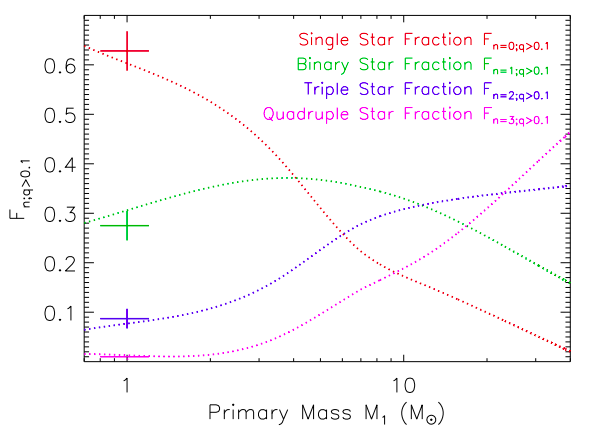
\includegraphics[width=\textwidth]{Thesis/figures/fig_moe_2017.png}
    \caption{Multiplicity fractions as a function of primary mass (dotted lines), including the single-star $F_{n=0;q> 0.1}$ (red), binary-star $F_{n=1;q> 0.1}$  (green), triple-star $F_{n=2;q> 0.1}$  (blue), and quadruple-star fraction $F_{n=3;q> 0.1}$  (magenta). Given a primary mass $M_1$, the model assumes that the multiplicity fractions follow a Poisson distribution across the interval $n = [0, 3]$ in a manner that reproduces the measured multiplicity frequency $F_{mult;q >0.1} = \Sigma_{n=1}^3 \; n F_{n;q> 0.1}$. For solar-type stars, this model matches the measured values (solid) within their uncertainties. Regardless of the uncertainties in the multiplicity fractions, $\leq 10\%$ of O-type stars are single while $\geq 55\%$ are born in triples and/or quadruples. Figure taken by \cite{moe2017mind}.}
    \label{fig:stellar_companions}
\end{figure}
The rich dynamical behavior of three-body systems can produce Lidov-Kozai cycles, in which the eccentricity of the inner orbit and the inclination between the inner and outer orbits vary periodically \citep{michaely2014secular,toonen2016evolution,mangipudi2022extreme}. As a result, tidal effects (tidal friction), gravitational-wave emission, and stellar interactions such as mass transfer, angular momentum exchange and collisions may be enhanced. In this way, evolution in triples can give rise to stellar mergers \citep{antonini2017binary,silsbee2017lidov,vigna2021massive}, namely some of most energetic events in the universe, ranging from gravitational wave sources to electromagnetic transients, e.g. luminous red novae, and also provide promising evolutionary pathways for exotic objects \citep{sana2012binary, toonen2016evolution}, e.g. blue stragglers \citep{winn2009spin}. In the past, most of our efforts in understanding the progenitors of the events were focused on modeling binary evolution disregarding the interaction of the binary with a third star. Therefore, a detailed examination of triple evolution is as necessary as it is challenging because it demands a self consistent treatment of three-body dynamics and stellar evolution.

In this thesis, I present the evolution of TIC 470710327 \citep{eisner2022planet}, a massive hierarchical triple system with a Roche lobe filling outer star. I use the Astrophysical Multipurpose Software Environment (AMUSE, \cite{portegies2018astrophysical}) to simulate the system's evolution and try to predict its future. Initially, I create stellar evolution models of the triple components until the tertiary fills its Roche lobe. I then simulate in detail the mass transfer for several orbits of the outer star using a combination of gravitational dynamics and hydrodynamics. I examine the importance of various parameters, properties and type of mass transfer, the response of the inner and outer orbital parameters, and the consequent evolution.

In the remainder of this first Chapter, I will present an overview of single massive star evolution until the end of helium burning phase with a focus on those aspects that are relevant for triple evolution. Furthermore, I will introduce concepts of binary evolution and I will argue how to extend these to the triple evolution case. After, presenting all the important concepts, I will introduce our target system, the goal and the outline of this project. 


\section{Goal \& Scientific Questions}

In this thesis, I present the evolution of TIC 470710327 \citep{eisner2022planet}, a massive hierarchical triple system with a Roche lobe filling outer star. I use the Astrophysical Multipurpose Software Environment (AMUSE, \cite{pelupessy2013astrophysical,portegies2018astrophysical}) to simulate the system's evolution and try to predict its future. Initially, I create stellar evolution models of the triple components until the tertiary fills its Roche lobe. I then simulate in detail the mass transfer for several orbits of the outer star using a combination of gravitational dynamics and hydrodynamics. 

There are two main scientific questions that I try to tackle:

\begin{itemize}
    \item How the mass transfer affects the orbital parameters of the two orbits?
    \item How the accretion of the binary affects the orbital parameters of the two orbits?
\end{itemize}

I examine the importance of various parameters, properties and type of mass transfer, the response of the inner and outer orbital parameters, and the consequent evolution.





\section{Thesis Outline}
This thesis is structured as follows: 

In the second chapter, I present an overview of single massive star evolution until the end of helium burning phase with a focus on those aspects that are relevant for triple evolution. Furthermore, I discuss concepts of binary evolution and I argue how to extend these to the triple evolution case. In the remainder of this chapter, I provide information about the scientific codes utilized in my simulations. In chapter three, I introduce my target system. In the fourth chapter, I display the setup of my simulations, the underlying assumptions of my models, and their physical justification.



%\subsection{AMUSE}

\section{Hierarchical Triple Star Systems}

\section{Goal and Outline of Thesis}

%\subsection{AMUSE}

\subsection{Thesis Outline}
This thesis is structured as follows: i








\chapter{Background}

\section{Evolution of Massive Stars in Isolation}\label{sec:single_star_evolution}

Stars with $M \leq 2$ M$_{\odot}$, $2 < M \leq 8$ M$_{\odot}$ and $M > 8$ M$_{\odot}$ are classified as low-, intermediate-, and high-mass, respectively. Despite the inherent rarity predicted by the initial mass function (IMF, see e.g. \cite{chabrier2005initial, dib2018emergence}), massive stars play a key role in the evolution of the Universe. They are the main source of UV radiation and heavy elements. They serve as a significant source of mixing and turbulence in the interstellar medium (ISM) of galaxies through a combination of winds, outflows, expanding HII regions, and supernova explosions. Galactic dynamos are powered by turbulence in conjunction with differential rotation. Cosmic rays are accelerated by the interaction of galactic magnetic fields and supernova shock fronts. The ISM is primarily heated by cosmic rays, UV radiation, and the dissipation of turbulence, whereas it is finally cooled by heavy metals present in dust, molecules, and in atomic/ionic form. Therefore, massive stars have a significant impact on galaxies' physical, chemical, and morphological structure \citep{kennicutt2005role}. However, the physical mechanisms behind the birth, development, and demise of massive stars remain elusive in comparison with low-mass stars \citep{zinnecker2007toward}. 


\subsection{Timescales of Stellar Evolution}

The fundamental timescales of stellar evolution are the dynamical ($t_{dyn}$), thermal ($t_{th}$), and nuclear timescales ($t_{nucl}$). The dynamical timescale is the characteristic time required for a star to collapse under its own gravitational force in the absence of internal pressure:

\begin{equation}
    t_{dyn} = \sqrt{\frac{R^3}{GM}} \sim 0.02 \left( \frac{R}{R_{\odot}} \right)^{3/2} \left( \frac{M}{M_{\odot}}\right)^{1/2} \; \text{days},
\end{equation}\label{eq:dynamical_timsecale}

where $R$ and $M$ are the star's radius and mass. It is a period on which a star might expand or contract if its hydrostatic equilibrium were disrupted, e.g. in case of sudden mass-loss.

Thermal (or Kelvin-Helmholtz) timescale indicates how quickly changes in a star's thermal structure may occur. It is therefore also the period on which a star responds when a its thermal equilibrium is disturbed:

\begin{equation}
    t_{th} = \frac{G M^2}{2RL} \sim 1.5 \times 10^7 \left( \frac{M}{M_{\odot}} \right)^{2} \frac{R_{\odot}}{R} \frac{L_{\odot}}{L} \; \text{yr},
\end{equation}\label{eq:thermal_timsecale}

where L is the star's luminosity.

Finally, the nuclear timescale corresponds to the time required for the star to exhaust its nuclear fuel supply at its current luminosity: 

\begin{equation}
    t_{nucl} = \frac{\phi M_{nucl} c^2}{L} \sim 10^{10} \frac{M}{M_{\odot}} \frac{L_{\odot}}{L} \; \text{yr},,
\end{equation}\label{eq:nuclear_timsecale}

where $\phi$ is the efficiency of nuclear energy production, $M_{nuc}$ is the amount of mass available as fuel, and $c$ is the light speed. For core hydrogen burning, $\phi = 0.007$ and $M_{nucl} \sim 0.1 M$.

Typically $t_{nucl} >> t_{th} >> t_{dyn}$, while assuming a mass-luminosity relation of $L \propto M^{\alpha}$, with empirically $\alpha \sim 3-4$ \citep{eker2015main}, it follows that massive stars live shorter and evolve faster than low-mass stars.

\subsection{Hertzsprung-Russell diagram}

The evolution of a star in isolation, namely single star evolution, is predominantly determined by the stellar mass. In their attempt to achieve hydrostatic and thermal equilibrium, stars generate temperatures and pressures that allow for nuclear burning. The cycles of nuclear burning and fuel exhaustion regulate the evolution of a star and set the various phases during the stellar lifetime. These burning cycles can be viewed as long-lived, but transient disruptions to a star's (or at least its core's) inexorable shrinkage under the effect of gravity. The virial theorem dictates this contraction is caused by the fact that stars are hot and lose energy through radiation. 
\begin{figure}[H]
    \centering
    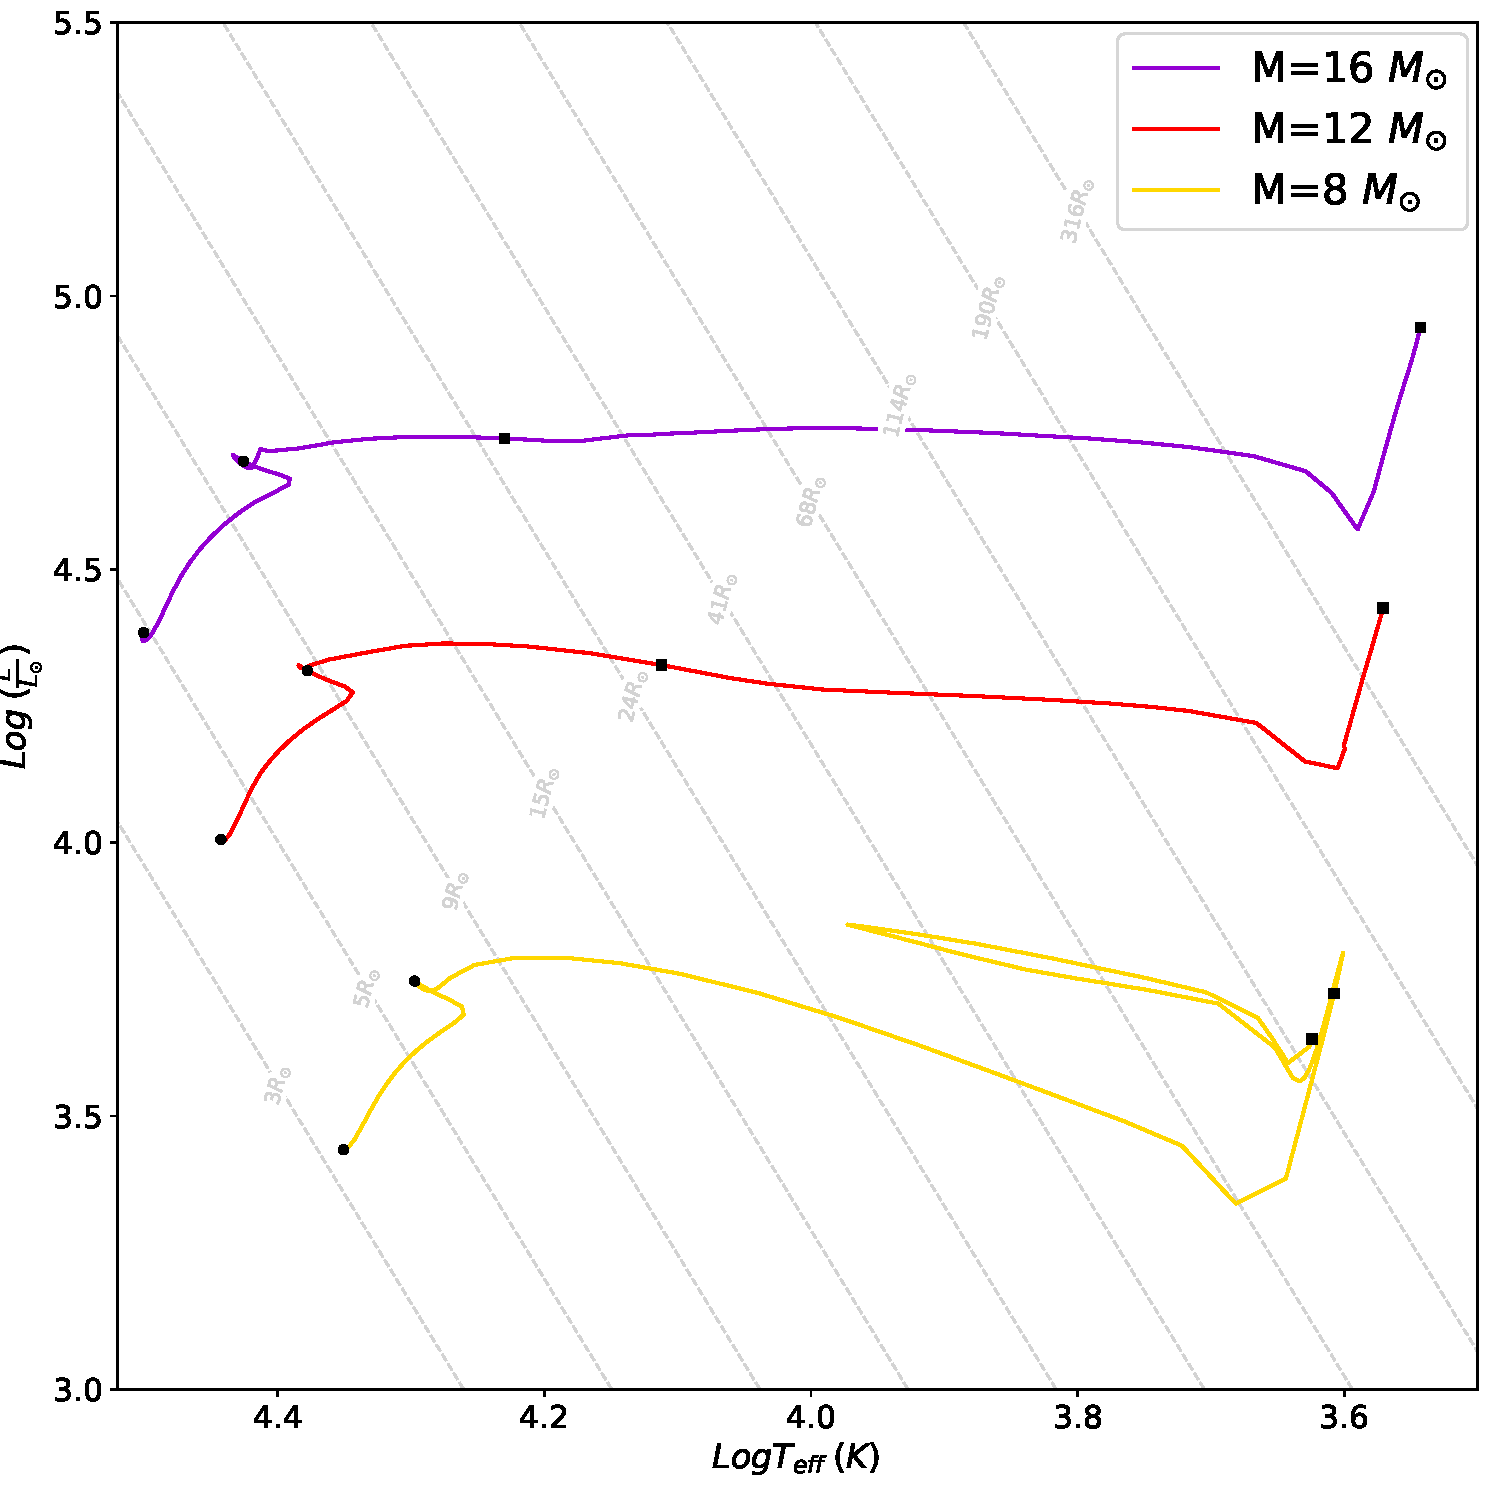
\includegraphics[width=0.9\textwidth]{Thesis/graphs/HR_massive_stars.pdf}
    \caption{Hertzsprung-Russell diagram. Evolutionary tracks for three stars with masses 8, 12 and 16 M$_{\odot}$ at solar metallicity until the end of Helium burning. Specific moments in the evolution of the stars are noted by black circles and squares as explained in the text. The tracks are calculated with MESA \citep{paxton2010modules,paxton2013modules,paxton2015modules,paxton2019modules}. The dashed lines show lines of constant radii by means of the Stefan–Boltzmann law.}
    \label{fig:HR_massive_stars}
\end{figure}
The Hertzsprung-Russell (HR) diagram in \cref{fig:HR_massive_stars} shows three evolutionary tracks for massive stars. The black circles correspond to the Zero Age Main Sequence (ZAMS) and the Terminal Age Main Sequence (TAMS). At ZAMS, the star having started the hydrogen burning in its core, achieves thermal equilibrium (TE), $L_{nuc}/L =1$, while TAMS is defined as the core hydrogen exhaustion point. Additionally, the black squares represent the start and end of helium burning in the core, respectively. In both cases the end of nuclear burning in the core is defined as the point when hydrogen and helium core mass fractions are $< 0.01$. The change in the star's physical radius occurs on different timescales depending on the physical mechanism buried beneath these processes. On nuclear timescale ($t_{nuc}$, see \eqref{eq:nuclear_timsecale}), stars evolve throughout the main sequence (MS) and the helium-burning phase, while on thermal timescale ($t_{th}$, see \eqref{eq:thermal_timsecale}), stars expand during the H-shell burning phase.

During the MS, hydrogen is fused into $^4$He. Independent of the ongoing reaction channel (pp or CNO), the luminosity of the star increases during this phase, (L$\,\propto\,\mu^{4}\,M^3$), due to the change in the core's composition ($\mu$ increases). Nevertheless, the way in which a star evolves through the MS-phase depends on its mass. Stars with masses M\,$\geq$\,1.3\,M$_\odot$, consequently massive stars too, are driven by the CNO-cycle ($\epsilon_{CNO}\,\propto\,\rho_{c}T^{18}_{c}$). The thermostatic action of the CNO-cycle causes the envelope to expand and, as a result, a decrease in effective temperature. Stars driven by the CNO-cycle evolve through larger radii and lower T$_{eff}$ than stars driven by the pp-cycle. Additionally, stars with masses M\,$\geq$\,1.3\,M$_\odot$ have convective cores, since the energy produced is too large to be transported by radiation ($\nabla_{rad} > \nabla_{ad}$). One effect of the convection on the evolution is that the MS-lifetime is extended (more detailed discussion in \cref{sub:mixing}). Another effect is that as the core approaches the end of H-burning, the reactions suddenly cease in the whole core, threatening the thermal equilibrium of the star. In response the temperature of the core needs to increase in order to keep the same energy generation rate leading to the contraction of the star. This is evident in the second part of the MS (see \cref{fig:HR_massive_stars}), where we observe the ``hook'' feature. 

At TAMS, where the hydrogen in the core has been depleted, hydrogen burning occurs in a shell around the core, while the central temperature is insufficient to initiate burning in the helium core. From that point on, the star enters the Hertzsprung gap branch and the evolution is driven by the mirror principle. The core contracts in $t_{th}$ in an attempt to reach thermal equilibrium, while the envelope expands. The aforementioned behavior is evident in Fig.\ref{fig:HR_massive_stars}, as the stars move towards bigger radius and lower effective temperature. An important thing to mention is that during this phase the temperature in the core is raising up and should not be confused with the effective temperature. Stars of less than $12$M$_{\odot}$ reach effective temperatures as low as ($10^{3.7}$K) 5000K before helium ignition. At this moment, they begin to ascend the red giant branch (RGB), which is accompanied by a significant rise in luminosity and radius. Due to the low effective temperature the opacity of the envelope rises and the latter becomes gradually convective. The prohibited zone of the HR-diagram is located to the right of the RGB, where hydrostatic equilibrium cannot be established. Any star in this zone will travel quickly towards the RGB. The red giant star has a compact core and an extensive envelope that extends hundreds of solar radii. When the temperature in the core exceeds $T_c \sim 10^8 K$, helium core burning begins, and the red giant phase ends. For stars with $M \geq 12$M$_{\odot}$, helium ignites before the effective temperature has dropped to a few thousand Kelvin. The stellar tracks for stars of less than $12$M$_{\odot}$ form a loop on the HR-diagram during helium burning, also known as the horizontal branch. The loop is accompanied by a drop and increase in the stellar radius. As the blazing front advances from the core to a shell enclosing the core, the star's outer layers expand again, and the evolution continues. For a more in depth description of the MS and post-MS evolution I direct the reader to \cite{pols2011stellar}.

\subsection{Stellar Winds}

Stellar winds play an important role in stellar evolution because they cause mass and angular momentum loss from the star. During the final stages of evolution on the AGB, low- and intermediate-mass stars experience significant mass-loss, which removes the remaining envelope, leaving only C-O white dwarfs as their final remnants \citep{marigo2007evolution}. On the other hand, for masses greater than 15 M$_{\odot}$, mass-loss by stellar winds becomes important during all evolution phases, including the main sequence. Observations in the ultraviolet and infrared spectrum show that these luminous massive stars experience rapid mass outflows (stellar winds) that can gradually erode their outer layers. For masses greater than 30 M$_{\odot}$, the mass-loss rates, $\dot{M}$, are so great that the mass-loss timescale, $t_{ml} = M / \dot{M}$, becomes shorter than the nuclear timescale, $t_{nuc}$. Even though stellar winds are fundamental in the formation and evolution of massive stars, the stellar wind mechanisms involved are not well understood in many cases. Hence $\dot{M}$ is frequently quite uncertain introducing significant uncertainties in the evolution of massive stars.

Driven by observations and theoretical models, stellar winds are usually in hot and cold winds because they are generated by different mechanisms. Numerous mass-loss rate prescriptions have been proposed, with $\dot{M}$ varying in different parts of the HR diagram. Hot, luminous massive stars (OB-type MS stars and blue supergiants, BSG) experience a stellar wind driven by radiation. Radiation pressure causes an outward acceleration at frequencies corresponding to absorption lines in the spectrum, where the interaction between photons and matter is strong. Because it is primarily the lines of the heavier elements that contribute to line driving, radiation-driven mass-loss is dependent also on metallicity \citep{vink2001mass}. Cool, luminous massive stars known as red supergiants (RSG) produce a stellar wind, which is likely caused by a combination of stellar pulsations and radiation pressure on dust particles that accumulate in the cool outer atmosphere, similarly with AGB stars. Because there are no theoretical predictions, empirical formulas that fit the average observed mass-loss rates of stars of roughly solar metallicity are used in theoretical studies. For example, mass-loss prescriptions based on \cite{reimers1975circumstellar,de1988mass,nieuwenhuijzen1990parametrization} are commonly used.

\subsection{Internal Mixing}\label{sub:mixing}

Even though the overall stellar evolution is only slightly affected by the initial chemical composition, a variety of internal mixing process can impact the life cycle, particularly of massive ($M>8$ M$_{\odot}$), stars \citep{langer2012presupernova}. Apart from convection, convective overshooting, semiconvection, and rotationally induced mixing are the most important internal mixing process \citep{schootemeijer2019constraining} and are still poorly understood. 

{\bf Convection}

{\bf Convective Overshooting}

Convective overshooting refers to the process of mixing beyond the boundaries of convective regions, which can occur when convective cells penetrate into radiative regions due to their non-zero velocity \citep{alongi1993evolutionary,brott2011rotating,schootemeijer2019constraining}. In stars with convective cores, e/g/ intermediate and massive stars, the size of the core is effectively enlarged through mechanisms such as convective core overshooting. This overshooting brings additional hydrogen into the core of the star and therefore directly impacts the final He core mass and main-sequence (MS) lifetime as well as the evolution of the stars after the MS.

{\bf Semiconvection}

{\bf Rotationally Induced Mixing}




\section{Binary Star Systems}

The evolution of a star in isolation could be summarized as: {\it Stars contract because they are hot and lose energy through radiation (Virial Theorem), while nuclear burning cycles serve as long-lived but transitory interruptions to a star's (or at least its core's) inevitable contraction due to gravity}. Despite that seemingly straightforward picture, massive stars tend form in multiple systems (see \cref{fig:stellar_companions}). Binaries particularly, which consist of two stars that orbit around a shared center of mass and are gravitationally connected to each other, are of immense importance. By nature,  they reveal more about themselves, particularly their masses and diameters, than other astronomical objects. This is especially true for eclipsing binaries \citep{prvsa2016physics}, which provide us with direct knowledge regarding spatial relations inside the source. Furthermore, close binaries are unique cosmic laboratories providing useful insights regarding different physical process. For example, gravitational wave emission is widely studied in binary mergers where both stars are compact objects \citep{cutler1994gravitational,abbott2017gw170608,abbott2019gwtc}, accretion as a power source in X-ray binaries \citep{lewin1997x,reig2011x}, while stellar interactions such as mass transfer, angular momentum exchange and tidal friction in close binaries {\it citation to be}. 

Despite the additional complexity that these stellar interactions provide to the evolution of these systems, they offer the necessary base for discussing stellar interactions in triple systems.  There are two fundamental reasons why many binaries transfer matter at some point in their evolution:

\begin{enumerate}
    \item During its evolution, one of the stars in a binary system may expand in radius (R$_{\star}$) or contract in binary separation (${\alpha}$) to the point where the companion's gravitational force can remove the outer layers of its envelope (Roche lobe overflow, RLOF).
    \item At some point in its evolution, usually during the late post-MS phases, one of the stars may release most of its mass in the form of a stellar wind; part of this material will be gravitationally trapped by the companion (stellar wind accretion). 
\end{enumerate}

This section is mainly focused on MS-MS interacting binaries via RLOF, (1). As discussed in \cref{sec:single_star_evolution}, this can occur because stars contract and expand during their evolution. Furthermore, the binary separation may decrease due to the loss of orbital angular momentum from the system as a result of stellar wind mass-loss or gravitational radiation. 

\subsection{Roche Lobe Overflow}

\subsubsection{Roche Lobes}

The evolution of binaries can be described by the stellar masses, $M_1$ and $M_2$, their orbital separation, $\alpha$, and the eccentricity, $e$, of their orbit \citep{postnov2014evolution,sana2012binary,toonen2014popcorn}.

\subsubsection{Conservative Mass Transfer}

\subsubsection{Non-Conservative Mass Transfer}


\section{Hierarchical Triple Star Systems}

\section{Scientific Codes}

In this section, I introduce the scientific codes that I coupled together in order to simulate the evolution of my target system.  Because these codes can be used in a variety of astrophysical scenarios, I will concentrate on their fundamental usage and working principles. I encourage users who want to dig deeper into the codes to follow the relevant citations.

\subsection{MESA}

MESA (Modules for Experiments in Stellar Astrophysics, \cite{paxton2010modules,paxton2013modules,paxton2015modules,paxton2019modules}) is a powerful and versatile 1D stellar evolution code that has become one of the most widely used tools in modern astrophysics. The code is designed to solve the fully coupled structure and composition equations simultaneously, allowing for highly accurate and detailed models of stars. MESA is written in Fortran and is developed and maintained by a large international collaboration of scientists.

MESA includes a wide range of physics modules for various astrophysical processes, such as the equation of state, nuclear reaction networks, hydrodynamics, convective and radiative energy transport, mass loss, rotation, and magnetic fields. The code can simulate the evolution of stars from their birth to their death, including complex phases such as helium and carbon burning, thermal pulses, and supernova explosions. As a result, MESA is an invaluable tool for astrophysical research, from studying the formation and evolution of stars to exploring the origins of the elements in the universe.

The central feature of MESA is the solution of the coupled structure and composition equations, which describe the internal structure of stars and the evolution of their chemical composition over time. These equations are based on fundamental principles of stellar physics, such as conservation of mass, momentum, and energy, as well as nuclear reactions that generate and consume energy in the star. The structure and composition equations can be written as a set of coupled differential equations that describe the evolution of the mass, radius, luminosity, temperature, and chemical composition of the star over time.

MESA also includes a comprehensive nuclear reaction network that describes the fusion of light elements into heavier elements in the stellar core. The network includes thousands of nuclear reactions that involve hundreds of isotopes, making it one of the most detailed and accurate nuclear reaction networks available for stellar evolution calculations.


\subsection{Gadget-2}

Gadget-2 (GAlaxies with Dark matter and Gas intEracT) is a smoothed particle hydrodynamics (SPH) code that simulates the gravitational and hydrodynamic evolution of collisionless and gaseous systems in astrophysical contexts. \citep{springel2005cosmological}. The code is capable of modeling a wide range of physical processes, such as gas dynamics, gravity, magnetic fields, and radiative transfer. Gadget-2 is written in C++ and is publicly available under the GNU General Public License.

The basic principle of the SPH method is to represent the fluid as a set of particles with associated physical attributes such as density, pressure, and velocity. To calculate these properties at a given point in space, the code uses a cubic spline kernel \citep{monaghan1985refined}, that is smooth and has a compact support, meaning it averages the properties of neighboring particles within a certain radius of the target point. Furthermore, the method is Lagrangian, meaning that the particles move with the fluid and do not have a fixed position in space.


The hydrodynamics computation in Gadget-2 is performed by solving the equations of motion for each particle in the simulation domain. The acceleration of each particle is calculated by summing the forces acting on it, including gravity, pressure gradients, and artificial viscosity. The gravity calculation uses the hybrid TreePM method \citep{bode2000tree,bagla2002treepm}, where the simulation volume is recursively subdivided into cubic cells, with each cell containing a maximum number of particles. The algorithm then builds a tree structure where each cell is treated as a node, and nodes that are spatially close are grouped together to form larger nodes. The final tree structure is used to compute the gravitational force on each particle avoiding the need to calculate the force between all pairs of particles in the system. This method reduces the computational cost from $O(N^2)$ for direct summation to $O(N\log N)$, where $N$ is the number of particles.


The code also includes modules for modeling magnetic fields and radiative transfer. The magnetic field module includes algorithms for calculating the magnetic field evolution and its effects on the gas dynamics. The radiative transfer module includes algorithms for calculating the transport of radiation through the simulation domain and its effects on the gas and dust properties. Gadget-2 can be run in parallel on high-performance computing clusters using the Message Passing Interface (MPI) standard.


\subsection{Huayno}

Huayno \citep{pelupessy2012n} is a high-performance N-body integrator code designed to simulate the dynamics of collisionless systems, such as galaxies, star clusters, and dark matter halos. The code is publicly available under the GNU General Public License and is written in C++. Similar with Gadget-2, the basic principle of Huayno is to use a hybrid algorithm \citep{bode2000tree} that combines the particle-mesh (PM) \citep{klypin1983three} and tree-based algorithms \citep{barnes1986hierarchical,dehnen2000very} to reduce the computational cost of simulating large systems.


The PM algorithm represents the gravitational potential as a discrete mesh of fixed resolution, and the particle positions are interpolated onto the mesh using a cloud-in-cell (CIC) scheme. The gravitational forces are then calculated by solving Poisson's equation on the mesh. The tree-based algorithm, on the other hand, uses a hierarchical structure to group particles into clusters and calculates the forces between clusters at different levels of the hierarchy. By combining the advantages of both algorithms, Huayno can handle a wide range of particle distributions and non-equilibrium systems, such as systems with binary or multiple stars.


Huayno also includes various subroutines and modules to facilitate the user in setting up simulations for different astrophysical scenarios. For example, the user can specify the initial conditions of the system, such as particle positions, velocities, masses, and physical properties. The user can also specify the boundary conditions of the simulation domain, such as periodic, reflecting, or outflow boundaries.

The code is designed to handle a wide range of particle distributions, from homogeneous and isotropic systems to anisotropic and structured systems. Huayno can also handle non-equilibrium systems, such as systems with binary or multiple stars. The user can specify the softening length of the gravitational interaction, which determines the spatial extent of the smoothing. The code also includes modules for integrating the orbits of particles, calculating the energy and angular momentum of the system, and analyzing the simulation output.

Huayno is designed to run efficiently on modern high-performance computing (HPC) clusters, and it supports parallel computing using the Message Passing Interface (MPI) standard. The code is optimized for a wide range of hardware architectures, including multi-core processors, GPUs, and FPGAs. The user can specify the number of processors or cores to use for the simulation, as well as the communication and load-balancing strategies.

In summary, Huayno is a powerful N-body integrator code that combines the PM and tree-based algorithms to simulate the dynamics of collisionless systems. The code is highly customizable and can handle a wide range of astrophysical scenarios, from galaxy formation to dark matter halos. The user can specify the initial conditions and boundary conditions of the simulation, as well as the softening length and other parameters. Huayno is optimized for parallel computing and can run efficiently on a wide range of HPC clusters.


\subsection{AMUSE}

Astrophysical Multipurpose Software Environment (AMUSE) is an open-source software package designed for astrophysical simulations and data analysis \citep{pelupessy2013astrophysical,portegies2018astrophysical}. The software is written in Python, which provides a user-friendly interface, and allows users to combine multiple astrophysical codes into a single simulation. AMUSE consists of a collection of modules that can be used to simulate a wide range of astrophysical phenomena, including stellar evolution, gravitational dynamics, hydrodynamics, radiative transfer, and cosmology.

One of the unique features of AMUSE is its ability to couple different simulation codes and to integrate them into a single framework. This allows researchers to simulate complex astrophysical phenomena that cannot be studied using a single code or method alone \citep{pelupessy2013astrophysical,portegies2018astrophysical}. For example, AMUSE can simulate the evolution of a binary star system, including the dynamics of the stars, the evolution of their interiors, and the transfer of mass and angular momentum between them. AMUSE can also simulate the formation and evolution of a star cluster, including the dynamics of the stars, the gas dynamics, and the radiative feedback from the stars.

AMUSE provides a powerful and flexible tool for data analysis, allowing users to analyze large data sets and to extract meaningful scientific results \citep{portegies2018astrophysical}. The software includes modules for data visualization, data reduction, and data analysis, allowing users to extract information from simulations and observational data.

AMUSE is designed to be highly scalable and can be run on a range of computing platforms, from laptops to high-performance computing clusters \citep{pelupessy2013astrophysical}. The software is optimized for parallel computing, and users can run simulations on multiple cores or distributed computing clusters using the Message Passing Interface (MPI) standard.

In summary, AMUSE is a powerful and versatile software package for astrophysical simulations and data analysis. The software allows researchers to simulate a wide range of astrophysical phenomena and to combine different simulation codes into a single framework. AMUSE provides a user-friendly interface and is highly scalable, making it an essential tool for astrophysical research in the era of big data.



\chapter{TIC 470710327}

\epigraph{The universe must be full of voices, calling from star to star in a myriad tongues. One day we shall join that cosmic conversation}{Arthur C. Clarke}

\chapter{Simulations}

%\epigraph{The stars are not distant objects to be admired from afar. They are our partners in exploration and discovery, and we must learn to live and work with them if we are to achieve our goals.}{Arthur C. Clarke}

The evolution of outer Roche lobe overflow (RLOF) triple-star systems is influenced by various physical processes, including stellar evolution, gravitational dynamics, and hydrodynamics. I utilize the Astrophysical Multi-purpose Software Environment (AMUSE, \cite{portegies2018astrophysical}), a comprehensive computational tool, to accurately simulate and solve for these physical processes in a self-consistent manner. To model the evolution of the system star prior to outer stars's RLOF, I employed a stellar evolution code (MESA, \cite{paxton2010modules,paxton2013modules,paxton2015modules,paxton2019modules}). Once the outer star reached the stage where it approximately filled its Roche lobe, I pause the stellar evolution simulation and converted the one-dimensional stellar structure into a three-dimensional hydrodynamical model. This hydrodynamical model of the outer star is then relaxed and placed in orbit around the binary star. Subsequently, I monitor the intricate hydrodynamics of the mass transfer from the Roche lobe-filling outer star to the inner binary for multiple orbits, while simultaneously keeping track of the gravitational dynamics of the three stars and the hydrodynamics of the gas from the outer star. A schematic representation of the entire process is provided in 

\section{Stellar Evolution}

MESA (Modules for Experiments in Stellar Astrophysics, \cite{paxton2010modules,paxton2013modules,paxton2015modules,paxton2019modules}) is an open-source 1D stellar evolution code used to model the evolution of stars from their birth to their death. It is a Fortran code that combines many numerical and physics modules for simulations of a wide range of stellar evolution scenarios ranging from very low mass to massive stars, including advanced evolutionary phases. Key modules within MESA include the equation of state module, the nuclear reaction network module, and the hydrodynamic module. MESA also includes modules for convective and radiative energy transport, as well as modules for mass loss, rotation, and magnetic fields. 

The code's basic principle is that it solves the fully coupled structure and composition equations simultaneously. Thus, allows me to track the independent evolution of the triple system components and obtain estimations of their properties at the moment of RLOF. In addition to fundamental parameters such as mass, radius, etc., MESA enables the access to the internal structure and detailed properties of the individual components. This information is essential for the conversion of one-dimensional stellar models into three-dimensional hydrodynamical realizations, providing a more comprehensive understanding of the physical processes involved in RLOF and the resulting mass transfer in these systems.

The stellar evolution calculations in this work are performed using the normal AMUSE parameters for MESA version 2208, with solar metallicity as the input. By the time the outer star approaches the radius of its Roche lobe, it has lost some mass and its radius is much bigger than when it was born. Table includes the important parameters of the system at the moment of RLOF. Figure 3 depicts the radial density profile of the outer component of the star at the moment of RLOF (green drawn line)





%\chapter{Hierarchical Triple Star Systems}



\newpage

\bibliographystyle{plainnat}
\bibliography{refs}

%## IMPORTANT#############################################
\acuseall
%## IMPORTANT#############################################

\end{document}